%        File: revise.tex
%     Created: Wed Oct 27 02:00 PM 2018 P
% Last Change: Wed Oct 27 02:00 PM 2018 P
%

%
% Copyright 2007, 2008, 2009 Elsevier Ltd
%
% This file is part of the 'Elsarticle Bundle'.
% ---------------------------------------------
%
% It may be distributed under the conditions of the LaTeX Project Public
% License, either version 1.2 of this license or (at your option) any
% later version.  The latest version of this license is in
%    http://www.latex-project.org/lppl.txt
% and version 1.2 or later is part of all distributions of LaTeX
% version 1999/12/01 or later.
%
% The list of all files belonging to the 'Elsarticle Bundle' is
% given in the file `manifest.txt'.
%

% Template article for Elsevier's document class `elsarticle'
% with numbered style bibliographic references
% SP 2008/03/01
%
%
%
% $Id: elsarticle-template-num.tex 4 2009-10-24 08:22:58Z rishi $
%
%
%\documentclass[preprint,12pt]{elsarticle}
\documentclass[answers,11pt]{exam}

% \documentclass[preprint,review,12pt]{elsarticle}

% Use the options 1p,twocolumn; 3p; 3p,twocolumn; 5p; or 5p,twocolumn
% for a journal layout:
% \documentclass[final,1p,times]{elsarticle}
% \documentclass[final,1p,times,twocolumn]{elsarticle}
% \documentclass[final,3p,times]{elsarticle}
% \documentclass[final,3p,times,twocolumn]{elsarticle}
% \documentclass[final,5p,times]{elsarticle}
% \documentclass[final,5p,times,twocolumn]{elsarticle}

% if you use PostScript figures in your article
% use the graphics package for simple commands
% \usepackage{graphics}
% or use the graphicx package for more complicated commands
\usepackage{graphicx}
% or use the epsfig package if you prefer to use the old commands
% \usepackage{epsfig}

% The amssymb package provides various useful mathematical symbols
\usepackage{amssymb}
% The amsthm package provides extended theorem environments
% \usepackage{amsthm}
\usepackage{amsmath}

% The lineno packages adds line numbers. Start line numbering with
% \begin{linenumbers}, end it with \end{linenumbers}. Or switch it on
% for the whole article with \linenumbers after \end{frontmatter}.
\usepackage{lineno}

% I like to be in control
\usepackage{placeins}

% natbib.sty is loaded by default. However, natbib options can be
% provided with \biboptions{...} command. Following options are
% valid:

%   round  -  round parentheses are used (default)
%   square -  square brackets are used   [option]
%   curly  -  curly braces are used      {option}
%   angle  -  angle brackets are used    <option>
%   semicolon  -  multiple citations separated by semi-colon
%   colon  - same as semicolon, an earlier confusion
%   comma  -  separated by comma
%   numbers-  selects numerical citations
%   super  -  numerical citations as superscripts
%   sort   -  sorts multiple citations according to order in ref. list
%   sort&compress   -  like sort, but also compresses numerical citations
%   compress - compresses without sorting
%
% \biboptions{comma,round}

% \biboptions{}


% Katy Huff addtions
\usepackage{xspace}
\usepackage{color}

\usepackage{multirow}
\usepackage[hyphens]{url}


\usepackage[acronym,toc]{glossaries}
%\newacronym{<++>}{<++>}{<++>}
\newacronym[longplural={metric tons of heavy metal}]{MTHM}{MTHM}{metric ton of heavy metal}
\newacronym{ABM}{ABM}{agent-based modeling}
\newacronym{ACDIS}{ACDIS}{Program in Arms Control \& Domestic and International Security}
\newacronym{ADS}{ADS}{Accelerator-Driven Systems}
\newacronym{AHTR}{AHTR}{Advanced High Temperature Reactor}
\newacronym{ANDRA}{ANDRA}{Agence Nationale pour la gestion des D\'echets RAdioactifs, the French National Agency for Radioactive Waste Management}
\newacronym{ANL}{ANL}{Argonne National Laboratory}
\newacronym{ANS}{ANS}{American Nuclear Society}
\newacronym{API}{API}{application programming interface}
\newacronym{ARE}{ARE}{Aircraft Reactor Experiment}
\newacronym{ARFC}{ARFC}{Advanced Reactors and Fuel Cycles}
\newacronym{ASME}{ASME}{American Society of Mechanical Engineers}
\newacronym{ASTRID}{ASTRID}{Advanced Sodium Technological Reactor for Industrial Demonstration}
\newacronym{ATWS}{ATWS}{Anticipated Transient Without Scram}
\newacronym{BDBE}{BDBE}{Beyond Design Basis Event}
\newacronym{BIDS}{BIDS}{Berkeley Institute for Data Science}
\newacronym{BWR}{BWR}{Boiling Water Reactor}
\newacronym{CAFCA}{CAFCA}{ Code for Advanced Fuel Cycles Assessment }
\newacronym{CDTN}{CDTN}{Centro de Desenvolvimento da Tecnologia Nuclear}
\newacronym{CEA}{CEA}{Commissariat \`a l'\'Energie Atomique et aux \'Energies Alternatives}
\newacronym{CI}{CI}{continuous integration}
\newacronym{CNEN}{CNEN}{Comiss\~{a}o Nacional de Energia Nuclear}
\newacronym{CNERG}{CNERG}{Computational Nuclear Engineering Research Group}
\newacronym{COSI}{COSI}{Commelini-Sicard}
\newacronym{COTS}{COTS}{commercial, off-the-shelf}
\newacronym{CSNF}{CSNF}{commercial spent nuclear fuel}
\newacronym{CTAH}{CTAHs}{Coiled Tube Air Heaters}
\newacronym{CUBIT}{CUBIT}{CUBIT Geometry and Mesh Generation Toolkit}
\newacronym{CURIE}{CURIE}{Centralized Used Fuel Resource for Information Exchange}
\newacronym{DAG}{DAG}{directed acyclic graph}
\newacronym{DANESS}{DANESS}{Dynamic Analysis of Nuclear Energy System Strategies}
\newacronym{DBE}{DBE}{Design Basis Event}
\newacronym{DESAE}{DESAE}{Dynamic Analysis of Nuclear Energy Systems Strategies}
\newacronym{DHS}{DHS}{Department of Homeland Security}
\newacronym{DOE}{DOE}{Department of Energy}
\newacronym{DRACS}{DRACS}{Direct Reactor Auxiliary Cooling System}
\newacronym{DRE}{DRE}{dynamic resource exchange}
\newacronym{DSNF}{DSNF}{DOE spent nuclear fuel}
\newacronym{DYMOND}{DYMOND}{Dynamic Model of Nuclear Development }
\newacronym{EBS}{EBS}{Engineered Barrier System}
\newacronym{EDF}{EDF}{Électricité de France}
\newacronym{EDZ}{EDZ}{Excavation Disturbed Zone}
\newacronym{EIA}{EIA}{U.S. Energy Information Administration}
\newacronym{EPA}{EPA}{Environmental Protection Agency}
\newacronym{EPR}{EPR}{European Pressurized Reactor}
\newacronym{EP}{EP}{Engineering Physics}
\newacronym{EU}{EU}{European Union}
\newacronym{FCO}{FCO}{Fuel Cycle Options}
\newacronym{FCT}{FCT}{Fuel Cycle Technology}
\newacronym{FEHM}{FEHM}{Finite Element Heat and Mass Transfer}
\newacronym{FEPs}{FEPs}{Features, Events, and Processes}
\newacronym{FHR}{FHR}{Fluoride-Salt-Cooled High-Temperature Reactor}
\newacronym{FLiBe}{FLiBe}{Fluoride-Lithium-Beryllium}
\newacronym{FP}{FP}{Fission Products}
\newacronym{GDSE}{GDSE}{Generic Disposal System Environment}
\newacronym{GDSM}{GDSM}{Generic Disposal System Model}
\newacronym{GENIUSv1}{GENIUSv1}{Global Evaluation of Nuclear Infrastructure Utilization Scenarios, Version 1}
\newacronym{GENIUSv2}{GENIUSv2}{Global Evaluation of Nuclear Infrastructure Utilization Scenarios, Version 2}
\newacronym{GENIUS}{GENIUS}{Global Evaluation of Nuclear Infrastructure Utilization Scenarios}
\newacronym{GPAM}{GPAM}{Generic Performance Assessment Model}
\newacronym{GRSAC}{GRSAC}{Graphite Reactor Severe Accident Code}
\newacronym{GUI}{GUI}{graphical user interface}
\newacronym{HLW}{HLW}{high level waste}
\newacronym{HPC}{HPC}{high-performance computing}
\newacronym{HTC}{HTC}{high-throughput computing}
\newacronym{HTGR}{HTGR}{High Temperature Gas-Cooled Reactor}
\newacronym{IAEA}{IAEA}{International Atomic Energy Agency}
\newacronym{IEMA}{IEMA}{Illinois Emergency Mangament Agency}
\newacronym{IHLRWM}{IHLRWM}{International High Level Radioactive Waste Management}
\newacronym{INL}{INL}{Idaho National Laboratory}
\newacronym{IPRR1}{IRP-R1}{Instituto de Pesquisas Radioativas Reator 1}
\newacronym{IRP}{IRP}{Integrated Research Project}
\newacronym{ISFSI}{ISFSI}{Independent Spent Fuel Storage Installation}
\newacronym{ISRG}{ISRG}{Independent Student Research Group}
\newacronym{JFNK}{JFNK}{Jacobian-Free Newton Krylov}
\newacronym{LANL}{LANL}{Los Alamos National Laboratory}
\newacronym{LBNL}{LBNL}{Lawrence Berkeley National Laboratory}
\newacronym{LCOE}{LCOE}{levelized cost of electricity}
\newacronym{LDRD}{LDRD}{laboratory directed research and development}
\newacronym{LFR}{LFR}{Lead-Cooled Fast Reactor}
\newacronym{LLNL}{LLNL}{Lawrence Livermore National Laboratory}
\newacronym{LMFBR}{LMFBR}{Liquid Metal Fast Breeder Reactor}
\newacronym{LOFC}{LOFC}{Loss of Forced Cooling}
\newacronym{LOHS}{LOHS}{Loss of Heat Sink}
\newacronym{LOLA}{LOLA}{Loss of Large Area}
\newacronym{LP}{LP}{linear program}
\newacronym{LWR}{LWR}{Light Water Reactor}
\newacronym{MAGNOX}{MAGNOX}{Magnesium Alloy Graphie Moderated Gas Cooled Uranium Oxide Reactor}
\newacronym{MA}{MA}{minor actinide}
\newacronym{MCNP}{MCNP}{Monte Carlo N-Particle code}
\newacronym{MILP}{MILP}{mixed-integer linear program}
\newacronym{MIT}{MIT}{the Massachusetts Institute of Technology}
\newacronym{MOAB}{MOAB}{Mesh-Oriented datABase}
\newacronym{MOOSE}{MOOSE}{Multiphysics Object-Oriented Simulation Environment}
\newacronym{MOX}{MOX}{Mixed Oxide Fuel}
\newacronym{MSBR}{MSBR}{Molten Salt Breeder Reactor}
\newacronym{MSRE}{MSRE}{Molten Salt Reactor Experiment}
\newacronym{MSR}{MSR}{Molten Salt Reactor}
\newacronym{NAGRA}{NAGRA}{National Cooperative for the Disposal of Radioactive Waste}
\newacronym{NEAMS}{NEAMS}{Nuclear Engineering Advanced Modeling and Simulation}
\newacronym{NEUP}{NEUP}{Nuclear Energy University Programs}
\newacronym{NFCSim}{NFCSim}{Nuclear Fuel Cycle Simulator}
\newacronym{NGNP}{NGNP}{Next Generation Nuclear Plant}
\newacronym{NMWPC}{NMWPC}{Nuclear MW Per Capita}
\newacronym{NNSA}{NNSA}{National Nuclear Security Administration}
\newacronym{NPRE}{NPRE}{Department of Nuclear, Plasma, and Radiological Engineering}
\newacronym{NQA1}{NQA-1}{Nuclear Quality Assurance - 1}
\newacronym{NRC}{NRC}{Nuclear Regulatory Commission}
\newacronym{NSF}{NSF}{National Science Foundation}
\newacronym{NSSC}{NSSC}{Nuclear Science and Security Consortium}
\newacronym{NUWASTE}{NUWASTE}{Nuclear Waste Assessment System for Technical Evaluation}
\newacronym{NWF}{NWF}{Nuclear Waste Fund}
\newacronym{NWTRB}{NWTRB}{Nuclear Waste Technical Review Board}
\newacronym{OCRWM}{OCRWM}{Office of Civilian Radioactive Waste Management}
\newacronym{ORION}{ORION}{ORION}
\newacronym{ORNL}{ORNL}{Oak Ridge National Laboratory}
\newacronym{PARCS}{PARCS}{Purdue Advanced Reactor Core Simulator}
\newacronym{PBAHTR}{PB-AHTR}{Pebble Bed Advanced High Temperature Reactor}
\newacronym{PBFHR}{PB-FHR}{Pebble-Bed Fluoride-Salt-Cooled High-Temperature Reactor}
\newacronym{PEI}{PEI}{Peak Environmental Impact}
\newacronym{PH}{PRONGHORN}{PRONGHORN}
\newacronym{PRIS}{PRIS}{Power Reactor Information System}
\newacronym{PRKE}{PRKE}{Point Reactor Kinetics Equations}
\newacronym{PSPG}{PSPG}{Pressure-Stabilizing/Petrov-Galerkin}
\newacronym{PWAR}{PWAR}{Pratt and Whitney Aircraft Reactor}
\newacronym{PWR}{PWR}{Pressurized Water Reactor}
\newacronym{PyNE}{PyNE}{Python toolkit for Nuclear Engineering}
\newacronym{PyRK}{PyRK}{Python for Reactor Kinetics}
\newacronym{QA}{QA}{quality assurance}
\newacronym{RDD}{RD\&D}{Research Development and Demonstration}
\newacronym{RD}{R\&D}{Research and Development}
\newacronym{RELAP}{RELAP}{Reactor Excursion and Leak Analysis Program}
\newacronym{RIA}{RIA}{Reactivity Insertion Accident}
\newacronym{RIF}{RIF}{Region-Institution-Facility}
\newacronym{SFR}{SFR}{Sodium-Cooled Fast Reactor}
\newacronym{SINDAG}{SINDA{\textbackslash}G}{Systems Improved Numerical Differencing Analyzer $\backslash$ Gaski}
\newacronym{SKB}{SKB}{Svensk K\"{a}rnbr\"{a}nslehantering AB}
\newacronym{SNF}{SNF}{spent nuclear fuel}
\newacronym{SNL}{SNL}{Sandia National Laboratory}
\newacronym{STC}{STC}{specific temperature change}
\newacronym{SUPG}{SUPG}{Streamline-Upwind/Petrov-Galerkin}
\newacronym{SWF}{SWF}{Separations and Waste Forms}
\newacronym{SWU}{SWU}{Separative Work Unit}
\newacronym{TRIGA}{TRIGA}{Training Research Isotope General Atomic}
\newacronym{TRISO}{TRISO}{Tristructural Isotropic}
\newacronym{TSM}{TSM}{Total System Model}
\newacronym{TSPA}{TSPA}{Total System Performance Assessment for the Yucca Mountain License Application}
\newacronym{ThOX}{ThOX}{thorium oxide}
\newacronym{UFD}{UFD}{Used Fuel Disposition}
\newacronym{UML}{UML}{Unified Modeling Language}
\newacronym{UNF}{UNF}{Used Nuclear Fuel}
\newacronym{UOX}{UOX}{Uranium Oxide Fuel}
\newacronym{UQ}{UQ}{uncertainty quantification}
\newacronym{US}{US}{United States}
\newacronym{UW}{UW}{University of Wisconsin}
\newacronym{VISION}{VISION}{the Verifiable Fuel Cycle Simulation Model}
\newacronym{VVER}{VVER}{Voda-Vodyanoi Energetichesky Reaktor (Russian Pressurized Water Reactor)}
\newacronym{VV}{V\&V}{verification and validation}
\newacronym{WIPP}{WIPP}{Waste Isolation Pilot Plant}
\newacronym{YMR}{YMR}{Yucca Mountain Repository Site}


\makeglossaries

%\journal{Annals of Nuclear Energy}

\begin{document}

%\begin{frontmatter}

% Title, authors and addresses

% use the tnoteref command within \title for footnotes;
% use the tnotetext command for the associated footnote;
% use the fnref command within \author or \address for footnotes;
% use the fntext command for the associated footnote;
% use the corref command within \author for corresponding author footnotes;
% use the cortext command for the associated footnote;
% use the ead command for the email address,
% and the form \ead[url] for the home page:
%
% \title{Title\tnoteref{label1}}
% \tnotetext[label1]{}
% \author{Name\corref{cor1}\fnref{label2}}
% \ead{email address}
% \ead[url]{home page}
% \fntext[label2]{}
% \cortext[cor1]{}
% \address{Address\fnref{label3}}
% \fntext[label3]{}

\title{Synergistic Spent Nuclear Fuel Dynamics Within the European Union\\
        \large Response to Review Comments}
\author{Jin Whan Bae, Clifford E. Singer, Kathryn D. Huff}

% use optional labels to link authors explicitly to addresses:
% \author[label1,label2]{<author name>}
% \address[label1]{<address>}
% \address[label2]{<address>}


%\author[uiuc]{Kathryn Huff}
%        \ead{kdhuff@illinois.edu}
%  \address[uiuc]{Department of Nuclear, Plasma, and Radiological Engineering,
%        118 Talbot Laboratory, MC 234, Universicy of Illinois at
%        Urbana-Champaign, Urbana, IL 61801}
%
% \end{frontmatter}
\maketitle
\section*{Review General Response}
We would like to thank the reviewers for their detailed assessment of
this paper. Your comments have resulted in changes which certainly improved the 
paper.


\section*{Reviewer 1}
\begin{questions}

        %---------------------------------------------------------------------
        \question Abstract. The abstract states that "These simulations 
        demonstrate that France can avoid deployment of additional LWRs by 
        accepting UNF from other EU nations, that lifetime extensions delay 
        time-to-transition, and improved breeding ratios are not particularly 
        impactful." These conclusions aren't highlighted or discussed properly 
        in the section of the report which presents the results and neither are 
        they highlighted in the conclusions.  

        \begin{solution}
        	Thank you for your valuable input. We performed an additional
        	analysis to find quantitative values representing the effect
        	of the change in breeding ratio and LWR lifetime extension.
                This quantitative assessment of the differential was described 
                via two new tables in the results section:
        	 
        	 \begin{tabular}{lrrrr}
        	 	\hline
        	 	  & \multicolumn{4}{c}{\% Difference} \\
                         \textbf{Breeding Ratio $\longrightarrow$}& \textbf{1.08}& \textbf{1.11} & \textbf{1.15} & \textbf{1.18} \\
        	 	\hline
        	 	Total reprocessing demand & 0.0 & -1.8 & -2.6 & -3.4 \\ 
        	 	LWR UNF reprocessed & 0.0  & -4.9 & -8.0 & -9.7 \\
        	 	\hline
        	 \end{tabular}
        	 
        	 \begin{tabular}{lrrrr}
        	 	\hline
        	 	& \multicolumn{4}{c}{\% Difference} \\
                         \textbf{LWR lifetime extension $\longrightarrow$}& \textbf{0 years}& \textbf{5 years} & \textbf{10 years} & \textbf{20 years} \\
        	 	\hline
        	 	Total reprocessing demand & 0.0 & -5.9 & -3.3 & 3.1 \\
        	 	LWR UNF reprocessed & 0.0  & 4.2 & 8.6 & 17.8 \\
        	 	\hline
        	 \end{tabular}

                 These were additionally noted in the conclusions with the 
                 following text: 
                 
                 The sensitivity study explored the effect of increased 
                 \gls{SFR} breeding ratio and existing \gls{LWR} lifetime 
                 extension. Increasing the breeding ratio reduced the amount of 
                 \gls{LWR} \gls{UNF} required to transition up to $9.7\%$ and 
                 decreased the total reprocessing demand up to $3.4\%$.  
                 Increasing the lifetime of existing \glspl{LWR} was not 
                 significant in reducing reprocessing demand, but provided the 
                 benefit of delayed transition.

        \end{solution}

        %---------------------------------------------------------------------
        \question In figures 2 and 3 the colour scheme makes it difficult to 
        distinguish the different data.
        \begin{solution}
        	Thank you for your input. We changed the color scheme so that
        	each component of the stacked chart can be more easily identified.
                Both impacted graphs have been altered with the new color 
                scheme below.

        	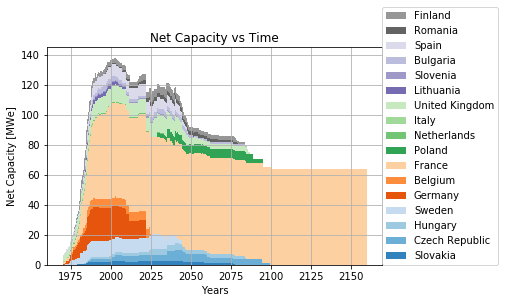
\includegraphics[width=0.7\textwidth]{../images/eu_future/onesim.png}

        \end{solution}

        %---------------------------------------------------------------------
        \question 1st sentence of Section 3 has been corrupted, with the ending 
        moved to the beginning.

        \begin{solution}
                Thank you for catching this error. The sentence has been corrected.
        \end{solution}

        %---------------------------------------------------------------------
        \question Table 4 and 5 both give imply U-235 compositions for PWR UOX 
        fuel with a low U-235 content of just 3.1 w/o. This is inconsistent 
        with the mean discharge burnups in the scenario, which would demand an 
        initial enrichment of about 4.5 w/o (this also reflects current 
        practice). If this interpretation is correct, it will affect the 
        simulation and could impact the results. I suspect that the same may 
        also apply to the BWR UOX fuel. 
        \begin{solution}
                Thank you for identifying this issue. You are correct. This was a clerical error. 
                We double checked the source of the fuel compositions to identify the
                initial enrichment used for generating the 51Gwd/MTHM burnup
                recipe, and the fresh fuel composition indeed had a higher
                enrichment, $4.29 \%$, than was assumed in the simulation 
                default parameters. Thank you again for your keen observation.
                We have made the changes in the paper and have re-run the 
                simulation with new input files. The only impacted parameter
                relevant to the study was the tails inventory and required 
                natural uranium feed. The simulated tails inventory
                and natural uranium both increased substantially ($\approx 
                24\%$).
        \end{solution}

        %---------------------------------------------------------------------
        \question Table 5 isn't referred to in the text.

        \begin{solution}
                There was a table with the same label in \LaTeX. Accordingly, 
                the reference in the text  to this table was misattributed. The 
                error is fixed and all tables are referred to in the text. 
                Thank you for catching this!
        \end{solution}

        %---------------------------------------------------------------------
        \question Paragraph immediately after Table 6 the text should read nine 
        tons of tails not nine times of tails.
        \begin{solution}
                Thank you for identifying this typo. This error is fixed.
        \end{solution}

        %---------------------------------------------------------------------
        \question Fig 10 caption: the correct spelling is usage

        \begin{solution}
                Thank you. This error is fixed.
        \end{solution}

        %---------------------------------------------------------------------
        \question Line 183 - corresponding is spelled incorrectly
        \begin{solution}
                Thank you for catching this. This error is fixed 
                (and a full spellcheck has been conducted).
        \end{solution}

        %---------------------------------------------------------------------
        \question Sections 6.1 and 6.2 should discuss the sensitivities to 
        breeding ratio and lifetime extension more completely and bring out the 
        conclusions noted in the abstract.

        \begin{solution}
                Thank you, we agree with this suggestion. We have added more quantitative
		analysis and discussion in sections 6.1 and 6.2 as well as the
		conclusion, as discussed in the response to comment 1 above.
        \end{solution}

        %---------------------------------------------------------------------
        \question Line 239 should read: ``The period during which ASTRID UNF.....
        \begin{solution}
                Thank you for your input. This error is fixed.
        \end{solution}

        %---------------------------------------------------------------------
        \question The conclusion should highlight the sensitivities to breeding 
        ratio and lifetime extension, as they are the main results from the 
        study.  

        \begin{solution}
                We agree. We have added this sentence in the conclusion:
                
                The sensitivity study explored the effect of increased SFR breeding
                ratio and existing LWR lifetime extension. Increasing the breeding
                ratio reduced the amount of LWR UNF required to transition
                up to $9.7\%$ and decreased the total reprocessing demand up to $3.4\%$.
                Increasing the lifetime of existing LWR was not significant
                in reducing reprocessing demand, but provided the benefit of delayed
                transition.
        \end{solution}


        \section*{Reviewer 2}


        %---------------------------------------------------------------------
        \question Overall, this paper does an excellent job of laying out its 
        modeling assumptions used to support their conclusions as to the 
        impacts of a spent fuel policy which would have France relying upon 
        international imports of UNF from EU member states to augment its 
        plutonium source material flows in order to "bootstrap" a fast reactor 
        transition policy. The use of data visualizations here is done quite 
        well, helping to visually guide the reader through the reasoning 
        process of the authors. In general, this is a thorough and 
        well-supported analysis which is worthwhile of publication.


        \begin{solution}
		Thank you for this thoughtful assessment. Bootstrap is a great
		word for this and we've replaced ``enable'' with ``bootstrap''
		in the abstract. 
        \end{solution}

        %---------------------------------------------------------------------
        \question First, in the introduction, it is stated, ``However, the 
        current inventory of French Used Nuclear Fuel (UNF) is insufficient to 
        fuel that transition without building new Light Water Reactors 
        (LWRs).''
        Is this conclusively established in the literature? (i.e., this seems 
        like it may be covered in refs. 4 and/or 5, but a little bit more 
        detail into how this conclusion has been reached / how limiting the 
        present policy is would be useful).
        \begin{solution}
                You raise an excellent point. Thank you. We have run an 
                additional simulation regarding just france, and have now added 
                the following figure, with some dicussion, as below:

                First, we confirmed that France does not have enough \gls{LWR} 
                \gls{UNF} to transition into a fully \gls{SFR} fleet. As shown 
                in figure (below). France cannot meet the 
                \gls{ASTRID} fuel demand without receiving \gls{LWR} \gls{UNF} 
                from other \gls{EU} nations. France is able to fuel some of its 
                \glspl{ASTRID} and breed more plutonium, but cannot meet the 
                fuel demand of all \glspl{ASTRID} with this aggressive 
                deployment scheme.  

		\includegraphics{../images/french-transition/france_only_compare.png}

	        Caption: \gls{ASTRID} fuel demand compared with fuel supply from only
			 France in the simulation. The lack of initial \gls{ASTRID} fuel
			 is caused by the lack of \gls{LWR} \gls{UNF} to reprocess. The
			 initial shortage then causes a decrease in plutonium bred by
			 \glspl{ASTRID}, thus a decrease in \gls{ASTRID} fuel supply.


        \end{solution}

        %---------------------------------------------------------------------
        \question Table 3 indicates a minimum UNF cooling time of 36 months; 
        yet on page 12 (line 120) the authors state a minimum residency time of 
        72 months. Which one was used?

        \begin{solution}
        	Thank you for noticing this ambiguity. Our intention was to have a 72-month
        	cooling time for LWR UNF, and a 36-month cooling time for SFR UNF.
        	This is now reflected and clarified in the revised version of
        	this paper.
        \end{solution}

        %---------------------------------------------------------------------
        \question In section 4.1 (Material Depletion), I appreciate the fact 
        that the authors have attempted to convey a realistic depletion-based 
        recipe for their materials. However, the means by which they reached 
        these values are unclear. Which version of Origen was used for this 
        depletion analysis? What assumptions were made with respect to the fuel 
        depletion? (i.e., what reactor libraries did the authors use to 
        calculate depleted inventories?) This latter question is important 
        particularly for establishing the isotopic vector of the MOX / ASTRID 
        fuel; i.e., how was the flux spectrum shape treated to calculate these 
        depletion values? This does not require an exhaustive recounting of the 
        methods here, but a simple discussion of how the authors arrived at 
        these results would aid in the reproducibility of this work. Similarly, 
        I'm assuming a uniform irradiation power for each batch (reasonable for 
        this type of project), but it may be useful to clarify. 
        \begin{solution}
                Thank you for pointing this out. The source of these recipes 
                was the \gls{AFCI} program libraries developed for fuel cycle 
                assessments in 2006 \cite{piet_fuel_2006}. The \gls{LWR} compositions 
                were calculated by \gls{ANL} personnel T.K. Kim as part of 
                Simulation, Evaluation, and Trade Study (SETS) work 
                package during FY2005 with followup work in FY2006. These 
                recipes, based on Appendix C of that document, were generated with 
                ORIGEN2, for high-burnup \gls{PWR} fuel using the one-group 
                cross sections that were provided with the code.  The high 
                burnup fuel has an initial enrichment of 4.2\% $^{235}U$ and a 
                discharge burnup of 50,000 MW-day/tonne. 


                Text regarding this has been added to Material Definitions 
                section thus:

                Reactor transmutation of the nuclear fuel was modeled using 
                isotopic `recipes', such that fresh and spent fuel recipes were 
                defined for each reactor type (see tables [fresh] 
                and [spent]).
                
                This work relied on reference \gls{LWR} \gls{UOX} and \gls{LWR} \gls{MOX} 
                compositions retrieved from \gls{AFCI} analyses in Appendix C 
                of \cite{piet_fuel_2006}.
                
                The \gls{LWR} \gls{UOX} depletion calculations were conducted 
                using ORIGEN2 with the \gls{PWR} one group cross sections 
                provided with ORIGEN2. Meanwhile, the \gls{LWR} \gls{MOX} 
                depletion calculations relied on WIMS8 \cite{wims8_wims_1999} 
                to provide accurate cross sections to ORIGEN. For this purpose, 
                WIMS8 calculations used the 172-group, JEF2.2-based cross 
                section library.

                Finally, the \gls{ASTRID} compostions were retrieved from the 
                \gls{ASTRID} design as published in 
                \cite{varaine_pre-conceptual_2012}.



        \end{solution}

        %---------------------------------------------------------------------
        \question For figures used to indicate sensitivities to modeling 
        assumptions (e.g., Figures 14, 15, 17, and 18). Here, I think 
        displaying these values as either a ratio to the baseline value or as a 
        net difference from the baseline would be more useful for conveying the 
        net effect; here, our interest in the effect at the margin, I would 
        assume, especially given that some of these differences are quite small 
        save for a short time period (e.g., the time region where the 
        decommissioning occurs). In as much, displaying these to represent the 
        differential effect (either through a net change or a ratio from the 
        baseline) would aid in highlighting the specific effect of these 
        assumptions which otherwise are somewhat obscured. If the authors feel 
        it necessary, a 2-axis design or a standalone articulation of these 
        throughputs for the baseline could easily support these figures if 
        showing the total throughput is required.)

        \begin{solution}
                Thank you for this detailed comment. Your insight is very 
                helpful here and also appeared in comments from Reviewer 1. To 
                highlight the important differential effect
                 more clearly, 
                we performed an additional
        	analysis to find quantitative values representing the effect
        	of the change in breeding ratio and LWR lifetime extension.
                This quantitative assessment of the differential was described 
                via two new tables in the results section:
        	 
        	 \begin{tabular}{lrrrr}
        	 	\hline
        	 	  & \multicolumn{4}{c}{\% Difference} \\
                         \textbf{Breeding Ratio $\longrightarrow$}& \textbf{1.08}& \textbf{1.11} & \textbf{1.15} & \textbf{1.18} \\
        	 	\hline
        	 	Total reprocessing demand & 0.0 & -1.8 & -2.6 & -3.4 \\ 
        	 	LWR UNF reprocessed & 0.0  & -4.9 & -8.0 & -9.7 \\
        	 	\hline
        	 \end{tabular}
        	 
        	 \begin{tabular}{lrrrr}
        	 	\hline
        	 	& \multicolumn{4}{c}{\% Difference} \\
                         \textbf{LWR lifetime extension $\longrightarrow$}& \textbf{0 years}& \textbf{5 years} & \textbf{10 years} & \textbf{20 years} \\
        	 	\hline
        	 	Total reprocessing demand & 0.0 & -5.9 & -3.3 & 3.1 \\
        	 	LWR UNF reprocessed & 0.0  & 4.2 & 8.6 & 17.8 \\
        	 	\hline
        	 \end{tabular}

                 These were additionally noted in the conclusions with the 
                 following text: 
                 
                 The sensitivity study explored the effect of increased 
                 \gls{SFR} breeding ratio and existing \gls{LWR} lifetime 
                 extension. Increasing the breeding ratio reduced the amount of 
                 \gls{LWR} \gls{UNF} required to transition up to $9.7\%$ and 
                 decreased the total reprocessing demand up to $3.4\%$.  
                 Increasing the lifetime of existing \glspl{LWR} was not 
                 significant in reducing reprocessing demand, but provided the 
                 benefit of delayed transition.
                
                
                \begin{tabular}{lrrrr}
                	\hline
                	\multirow{2}{*}{\textbf{Parameter}} & \multicolumn{4}{c}{\% Difference} \\
                	& \textbf{1.08}& \textbf{1.11} & \textbf{1.15} & \textbf{1.18} \\
                	\hline
                	Total reprocessing demand & 0.0 & -1.8 & -2.6 & -3.4 \\ 
                	LWR UNF reprocessed & 0.0  & -4.9 & -8.0 & -9.7 \\
                	\hline
                \end{tabular}
                
                	\begin{tabular}{lrrrr}
                		\hline
                		\multirow{2}{*}{\textbf{Parameter}} & \multicolumn{4}{c}{\% Difference} \\
                		& \textbf{base}& \textbf{5 years} & \textbf{10 years} & \textbf{20 years} \\
                		\hline
                		Total reprocessing demand & 0.0 & -5.9 & -3.3 & 3.1 \\
                		LWR UNF reprocessed & 0.0  & 4.2 & 8.6 & 17.8 \\
                		\hline
                	\end{tabular}
                
        \end{solution}

        %---------------------------------------------------------------------
        \question Line 58: Megawatt is one word
        \begin{solution}
                This error is fixed.
        \end{solution}

        %---------------------------------------------------------------------
        \question Line 133: This section begins with a sentence fragment.

        \begin{solution}
                We have changed the sentence 
                "The scenario specifications defining the simulations
                presented in this work are listed in table 3."
                to
                "Table 3 lists the scenario specifications defining the
                simulations presented in this work."
        \end{solution}


        \section*{Reviewer 3}
        %---------------------------------------------------------------------
        \question Very nice approach of extracting realistic reactor data from 
        PRIS database and thorough literature review of other fuel cycle data
        \begin{solution}
                Thank you.
        \end{solution}


        %---------------------------------------------------------------------
        \question There's no explanation for why ASTRID reactors would last 80 
        years

        \begin{solution}
                The ASTRID design target is 60 years \cite{gauche_generation_2012},
                but we assumed a lifetime
                extension of 20 years, considering that most French nuclear reactors
                have their lifetimes extended. We assume that technological
                advances in materials and design will allow 80-year lifetimes
                for ASTRID reactors. We have added the following text to the 
                paper:


The \gls{ASTRID} design targets a 60 year lifetime \cite{gauche_generation_2012}.
We assume technology and material robustness improvements before deployment in 2040.
Accordingly, we optimistically assume an 80 year lifetime instead, reflecting 20 year
lifetime extensions for each \gls{ASTRID} reactor in 2100 and beyond.

        \end{solution}

        %---------------------------------------------------------------------
        \question Varying the lifetime extension via random sampling is very 
        innovative
        \begin{solution}
                Thank you !
        \end{solution}

        %---------------------------------------------------------------------
        \question How was the 36 month minimum cooling time decided? LWR UNF 
        typically requires 5 years before decay heat sufficiently low for 
        transport and for PUREX process

        \begin{solution}
                Thank you for your input. Our intention, reflected in our 
                simulations, was to have a 72-month
                cooling time for LWR UNF, and a 36-month cooling time for SFR UNF.
                This is now reflected and clarified in the revised version of
                this paper everywhere these durations are mentioned.
        \end{solution}

        %---------------------------------------------------------------------
        \question page 16, line 17, duplicate "recipe"
        \begin{solution}
                Thank you for your input. This error is fixed.
        \end{solution}

        %---------------------------------------------------------------------
        \question Are the first SFR cores loaded entirely with fresh 
        equilibrium fuel? At 22\% Pu?  If so, this will overpredict first core 
        fissile requirements. If not, then there should be emphasis on how the 
        initial core has different fuel zones with various Pu contents 
        simulating burned fuel (at 13\%, 16\%, 19\%, 22\%, for example)

        \begin{solution}
                Thank you for this detailed insight. Of course, you are quite right. 
                We did originally assume
                that the first SFR cores are loaded entirely with
                fresh equilibrium fuel at 22\% Pu. However, we also assumed
                that the core size is set so that the initial plutonium
                loading (at 22\% enrichment) is 4.9 tons, as stated in
                literature \cite{chenaud_status_2013}. Thus, we are
                actually overpredicting the later refuel batch fissile
                requirements by 74.9 kg ($\approx$ 6\%). 
                Ideally, as you mentioned, the initial fuel loading
                could be represented more faithfully with regard to initial
                fuel zones.
                This can be accomplished with the Cyclus simulator 
                and Cycamore Reactor archetype, but will require depletion 
                calculations outside of the current scope of this effort. We 
                have listed your suggestion as potential future work as it 
                would certainly improve the fidelity of future results.     
        \end{solution}


        %---------------------------------------------------------------------
        \question The estimated 200 SFRs that can be started up with the 985 
        tPu does not take into account the reload fuel required to sustain the 
        first SFRs until they can recycle their own fuel (which may take a few 
        years). Perhaps this is why Cyclus calculated 180 SFRs started up 
        instead of 200. The startup reload fuel requirements should also be 
        mentioned in addition to the startup first core requirements.
        \begin{solution}
                You are indeed correct. The 200 SFR calculation was
                simply an algebraic calculation:
                \[ \frac{985 tPu}{4.9 tPu per SFR} \approx 200 \]
                But we do understand that it is confusing for the reader
                to see this sentence, so we removed it since it does not
                contribute to the flow or conclusions of the paper.
        \end{solution}

        %---------------------------------------------------------------------
        \question Several typos spotted. Run spell check and proof read.

        \begin{solution}
                Thank you for noticing these issues. We apologize that these 
                snuck past our initial review. We have conducted an additional
                grammar and spelling check to catch these errors.
        \end{solution}

        %---------------------------------------------------------------------
        \question Did you just artificially change the breeding ratio of the 
        SFR without design considerations?  i.e., changes in core size, 
        spectrum, burnup, Pu content, etc. If so, these results may not be 
        valid.  If not, please include descriptions of the SFR core 
        modifications made to enable the different breeding ratios. If the 
        excess reactivity decreases from BOC to EOC, then an increase in the 
        breeding ratio may result in larger initial core Pu mass requirements.
        \begin{solution}
                Thank you. Your point is quite correct. 
                Yes, we did just artificially change
                the breeding ratio of the SFR without design considerations.
                The are large uncertainties introduced with this arbitrary
                breeding ratio increase, and we have now suggested your
                ideas as future work. This section of the analysis intends
                only to identify first-order trends. The simulation itself
                involves many simplifying assumptions regarding both 
                policy and reactor physics. Accordingly, while individual 
                depletion calculations regarding various breeding ratios 
                would improve precision, it may not improve accuracy.
        \end{solution}

        %---------------------------------------------------------------------
        \question Can you show a figure of surplus separated Pu or surplus LWR 
        UNF for the scenario to show how much margin there is? It is stated 
        that there is enough Pu from the LWR UNF to start the SFR fleet, but by 
        how much?
        \begin{solution}
	        	Thank you for this great idea.
                We added a paragraph describing the surplus:
                
                If France receives LWR UNF from all EU nations,
                except Sweden and Finland, due to their concrete waste management plan,
                it will have a surplus of $30,648$ MTHM of LWR UNF. This
                inventory can be leveraged to increase French nuclear power capacity as
                the transition takes place. However, pragmatic limitations such
                as new reactor construction, reprocessing throughput, and
                political / economical concerns remain. 
                
        \end{solution}



        %---------------------------------------------------------------------
\end{questions}
\bibliographystyle{unsrt}
\bibliography{revise}
\end{document}

  %
  % End of file `elsarticle-template-num.tex'.
